\documentclass[12pt]{report}


\usepackage[utf8x]{inputenc}
\usepackage[T1]{fontenc}
\usepackage{textcomp}
\usepackage{eurosym}
\usepackage[frenchb]{babel}

\usepackage{graphicx}

\usepackage{todonotes}
\usepackage{pdfcomment}

\usepackage{hyperref}
\usepackage[all]{hypcap}
\hypersetup{
    colorlinks,
    linkcolor={red},
    citecolor={blue!50!black},
    urlcolor={blue!80!black}
}
\def\subsectionautorefname{section}

% Title Page
\title{Rapport de stage Technique:
	Neurospin}
\author{Christophe Launay, Promo 2015, M1, EFREI\\
	Tuteur : Dr Sliman, Maitre de stage : Dr Houenou \& Dr Duchesnay}

\newcommand{\comment}[2]{\pdfcomment[author=#1]{#2}}
\newcommand{\filename}[1]{\texttt{#1}}

\begin{document}
	
\maketitle

\tableofcontents

\chapter*{Introduction}
\addcontentsline{toc}{chapter}{Introduction}

Ce rapport vous présentera l'ensemble de mon stage technique effectué lors de ma première année de master au sein de l'EFREI. Ce stage a été effectué au CEA (Commissariat à l'Énergie Atomique), et plus précisément à Neurospin, laboratoire de recherche en neuro-imagerie. 
Durant ce stage, j'ai effectué des recherches sur la prédiction des troubles bipolaires et le sujet qui m'a été confié est le suivant : \\

Écrire un script python afin d'exécuter un script d'apprentissage artificiel afin de pouvoir prédire sur une population donnée quel sujet est atteint de bipolarité. \\


Ce rapport vous présentera Neurospin, puis le sujet avec son cahier des charges, les méthodes utilisées pour comprendre l'apprentissage artificiel, comment le script a été conçu et pour quelles raisons.
Après cela, je présenterai l'analyse et l'explication des résultats.
Pour finir, je présenterai le bilan du stage, ce que j'ai appris, les problèmes rencontrés et comment ils ont été résolus. 


\chapter{Neurospin et son environnement}



\section{Neuropsin}

NeuroSpin est une grande infrastructure de neuro-imagerie située à l’intérieur du CEA de Saclay. Ce centre possède des imageurs à résonance magnétique à champ intense et vise à repousser les limites actuelles de l’imagerie cérébrale. Tout d’abord, on ne peut parler de NeuroSpin sans aborder le bâtiment en lui-même. En effet, ce bâtiment très impressionnant, imaginé par Claude VASCONI, a mis deux ans à sortir de terre. Les travaux ont commencé en janvier 2005 et les locaux ont commencé à être utilisés depuis le 1er janvier 2007. Ce bâtiment, fait de béton, d’acier et de verre, forme un ensemble linéaire composé de deux édifices parallèles, de part et d’autre d’une nef centrale de 135 mètres de long, appelée encore ‘galeria’. Cette nef, véritable colonne vertébrale de l’édifice, est conçue comme un espace de rencontres entre les différentes équipes de chercheurs. NeuroSpin s’étend sur environ 11 400m².

L’édifice Ouest, dont la façade est composée de structures sinusoïdales entièrement métalliques, est développé uniquement en rez-de-chaussée et contient les ensembles de recherche clinique, de recherche pré-clinique (des lits sont installés pour accueillir des patients) et les salles des aimants abrités dans des alcôves magnétiquement confinées.

Un sous-sol partiel est réservé à l’usage des locaux techniques et locaux de stockage.
Une voie d’accès raccordée à l’entrée Est du Centre dessert le bâtiment et le parking extérieur de 100 places.

Le centre NeuroSpin est dirigé par M. Denis LE BIHAN élu à l'académie des sciences et chevalier de l'Ordre national du mérite.


\section{La hiérarchie}

présentation de la hiérarchie Neurospin
\section{Résumé}

\underline{NeuroSpin en quelques dates :}

\begin{itemize}
	\smallskip
	\item Remise des études de faisabilités industrielles : juillet 2004
	\item Permis de construire : septembre 2004
	\item Début des travaux : janvier 2005
	\item Livraison du 3T : mai 2006
	\item Inauguration du bâtiment : juin 2006
	\item Livraison du 7T : août 2006
	\item Livraison du 11,7T : 2010/2011
	\item Installation du 11,7T : 2014 
\end{itemize}
\medskip

\underline{Côté technique :}

\begin{itemize}
	\smallskip
	\item  Architecte : Claude Vasconi
	\item  Surface : 11 400 m²
	\item  Début des travaux : janvier 2005
	\item  Début de l’exploitation : 1er janvier 2007
	\item  150 personnes attendues : médecins, pharmaciens, mathématiciens, physiciens, …
\end{itemize}
\medskip

\underline{Côté finances (coût du bâtiment et des aimants à ce jour) :}

\begin{itemize}
	\smallskip
	\item CEA : 33,3 M\euro
	\item ANR (Agence Nationale de la Recherche) : 10 M\euro
	\item Conseil régional d’Ile-de-France : 6 M\euro
	\item Conseil général de l’Essonne : 1,7 M\euro
\end{itemize}


\chapter{Présentation du projet et cahier des charges}

% Étude du trouble bipolaire par l'imagerie de diffusion.
Le projet consiste à déterminer, à partir d'un examen d'Imagerie par Résonance Magnétique (IRM), si des patients sont atteints de trouble bipolaire ou non.
La motivation pour cette étude est que ces examens sont indolores et rapides.
Pour cela, nous utilisons des techniques d'apprentissage artificiel (appelé \textit{Machine Learning} en anglais).
De plus, grâce à ces techniques, on peut étudier quelles régions du cerveau sont impliquées dans la maladie et ainsi
obtenir des marqueurs biologiques de la maladie (\textit{biomarkers} en anglais).

Nous avons travaillé avec une modalité d'IRM particulière appelée IRM de diffusion (\textit{Diffusion Weighted Imaging (DWI)} en anglais)
que nous présentons brièvement dans la~\autoref{sec:dwi}.

\section{Les troubles bipolaires : explication}

Pour bien comprendre la nature de la recherche, il faut savoir ce que sont les troubles bipolaires. Une bipolarité est un trouble mental qui influe sur l'humeur, oscillant entre des périodes de dépression et d'hypomanie (élévation de l'humeur) avec entre les deux, des périodes d'humeur "normale" (euthymie).


\section{DWI : Diffusion Weighted Imaging} \label{sec:dwi}

L'IRM de diffusion est une technique basée sur l'imagerie par résonance magnétique (IRM).
Elle permet de mesurer en chaque point du volume imagé la distribution des directions de diffusion des molécules d'eau à l'intérieur du cerveau.
La diffusion des molécules d'eau est contrainte par les tissus environnants, cette modalité d'imagerie permet d'obtenir indirectement la position, l'orientation et l'anisotropie des structures fibreuses, notamment les faisceaux de matière blanche du cerveau.
L'hypothèse qui sous-tend le projet est que des changements dans la matière blanche peuvent indiquer des changements pathologiques.

\section{Présentation du projet}

% \comment{Mathieu}{Cette partie n'est pas très claire. Je pense qu'il ne faut pas parler ici des échantillons d'apprentissage et de tests.
%                   En revanche, tu peux dire ce qui était présent au début du projet: données cliniques et images provenant de différents centres, avec les données
%                   des identifiants différents et un ordre différent.
%                   Ainsi, tu justifie la première partie du cahier des charges.
%                   De plus, tu peux dire qu'on utilise un modèle doté de nombreux paramètres et donc qu'on va devoir essayer beaucoup de combinaisons.
%                   Comme chaque évaluation est lourde (validation croisée), ça nécessite l'emploi d'un cluster et des logiciels développés à NS pour ça.
%                   Il faut aussi évoquer les différentes hypothèses (différents masques et images squeletissées).
%                   La partie 4 donne des détails qui peuvent être intéressants ici.
%                   Voir les remarques en section 4}

Afin d'étudier la maladie, une base de données contenant des patients atteints de bipolarité et des sujets sains (sujets contrôle) a été constituée
en collaboration entre plusieurs hôpitaux en France, en Allemagne et aux États-Unis.
Ces sites nous ont fourni les données cliniques de chaque sujet ainsi que leur IRM respectif.
% Compte tenu du fait que les données proviennent de 3 sites différents, les identifiants des sujets ne correspondent pas toujours aux a ceux des images IRM ou bien l'ordre est différent ou bien il y a des données manquantes, etc... 
% Suite à la résolution de ces différents problèmes, nous étudions ces données avec un modèle estimateur qui possède 5 hypers-paramètres (K, $\alpha$, l1, l2, tv). Chacun de ces paramètres possède plusieurs valeurs et chacune des combinaisons de ces 5 valeurs seront testées ce qui correspond a 2475 combinaisons. 

Nous voulons évaluer un algorithme d'apprentissage développé à Neurospin.
Cet algorithme possède de nombreux paramètres.
Nous voulons donc trouver la meilleure combinaisons de ces paramètres.

Comme nous avons beaucoup de combinaisons à tester et que la méthode d'évaluation est lourde,
nous utiliserons un cluster et des logiciels développés par Neurospin afin de paralléliser l'évaluation.

Nous voulons de plus tester plusieurs hypothèses scientifiques telles que:
\begin{itemize}
	\item l'influence d'autres variables telles que le sexe, l'âge ou le scanner IRM utilisé
	\item la restriction a une partie du cerveau afin de focaliser notre analyse sur des régions précises du cerveau
	\item l'utilisation de pré-traitement supplémentaire (squeletisation) sur les images
\end{itemize}

% Le sujet de ce programme repose sur différentes hypothèses : 
% \begin{enumerate}
% 	\item les images initiales et une matrice avec le sexe et l'age auquel l'image a été prise l'IRM sans intercept.
% 	\item les images initiales avec une matrice au mêmes covariables avec l'intercept. 
% 	\item les deux premières hypothèses mais avec des images squeletonisées.
% 	\item Les images de bases avec une covariable en plus : les sites ont été rajoutés
% 	\item un masque tronqué d'une partie du cerveau afin de focaliser notre analyse sur des régions précises du cerveau.  
% \end{enumerate}
% 
% les hypothèses sans intercept et sans sites ne seront pas présentés dans ce rapport pour raison de résultat insatisfaisant. 

\section{Le cahier des charges}

Une présentation des différentes étapes qui vont mener à la prédiction des résultats :

\begin{itemize}
 \item Construction de la population: fusionner la liste des images et les données cliniques
 \item Mise en forme des images et des variables d'intérêt pour leur utilisation par l'algorithme d'apprentissage
 \item Paramétrer et lancer les calculs sur le cluster
 \item Interprétation
\end{itemize}

Pour continuer sur la mise en œuvre de ce projet, un peu de théorie concernant les méthodes utilisés. 

\chapter{Méthodes}

Ce chapitre fournit des explications sur les méthodes d'évaluation et de calcul utilisées dans le projet.



\section{Apprentissage artificiel}

\comment{}{Présentation plus générale s'inspirant de http://fr.wikipedia.org/wiki/Apprentissage_supervis\%C3\%A9. Note qu'il existe aussi un apprentissage non-supervisé qu'on ignore ici.}

D'un point de vue informatique, un algorithme d'apprentissage peut être vu comme un objet doté de 2 types de paramètres:
\begin{itemize}
 \item des paramètres dépendant des données qu'on va estimer à partir de données d'apprentissage notés $\theta$
 \item des paramètres fixés à la création de l'objet appelés hyper-paramètres
\end{itemize}
Son utilisation se fait en 2 phases:
\begin{itemize}
 \item une phase d'apprentissage (voir~\autoref{fig:Apprentissage_Machine}) au cours de laquelle on va estimer les paramètres $\theta$ grâce à 2 jeux de données:
       une matrice $X_{train}$ qui représente les données et une matrice $y_{train}$ qui représente les résultats correspondant aux données.
       On cherche en général des paramètres qui permettent d'optimiser un certain critère, notés $\theta^{*}$.
       Cependant, l'algorithme ne fournit pas en général les paramètres optimaux mais une approximation notée $\hat{\theta}$.

 \item une fois l'apprentissage effectué, on peut utiliser l'algorithme pour prédire les labels $y_{pred}$ associés à de nouvelles données $X_{test}$ (voir~\autoref{fig:Apprentissage_Machine_Prediction}).
\end{itemize}

\begin{figure}[htpb]
	\centering
	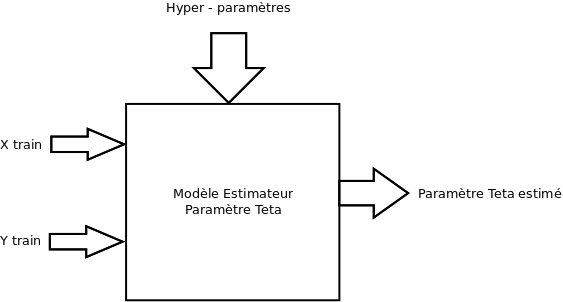
\includegraphics[scale = 0.25]{images/Diagramme1}
	\caption{Représentation de la phase d'apprentissage.}
	\label{fig:Apprentissage_Machine}
\end{figure}

% Ici, l'estimation du paramètre $\theta$ doit être tel que l'erreur estimé sur les prédictions soit le minimum possible. 
% Cette erreur est estimée selon un modèle de régression linéaire qui doit minimiser selon le paramètre $\theta$ par la méthode des moindres carrés, c'est-à-dire minimiser la formule suivante : 
% 
% \begin{equation}
% erreur = \sum_{i=1}^{n} (|y_{i} - \hat{y}_{i}|^{2})
% \end{equation}
% avec $y_{i}$ les vrais résultats et $\hat{y}_{i}$ les résultats estimés. 
% 
% Une fois que l'erreur a été estimé et que les $\theta$ ont été calculé, il est testé sur un échantillon test, suite à cela, la machine calcul une prédiction des résultats qu'on compare aux vrais résultats (voir~\autoref{fig:Apprentissage_Machine_Prediction}). 

\begin{figure}[htpb]
	\centering
	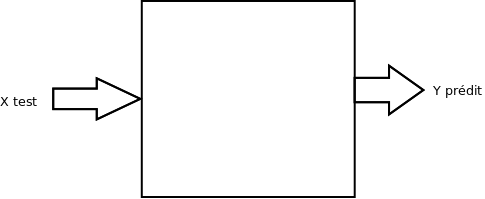
\includegraphics[scale = 0.25]{images/App_Mach_Prediction}
	\caption{Utilisation d'un algorithme pour la prédiction de nouvelles données.}
	\label{fig:Apprentissage_Machine_Prediction}
\end{figure}

\todo{expliquer l'apprentissage des k voxels}

\section{Modèle}

Notre estimateur consiste à effectuer une régression logistique afin de trouver le vecteur de poids $\beta$ (ici, $\beta$ = $\theta$).
Dans un premier temps, une régression linéaire est effectuée et par dessus celle-ci, une fonction logistique est appliquée afin de classer les résultats à 0 ou 1. 

\subsection{Filtre univarié}

On fait un test F de Fisher sur chaque voxel pour savoir si il prédit bien le statut clinique.
On sélectionne les k meilleurs.

\subsection{Régression Logistique}

% La régression linéaire consiste à calculer une droite qui passe au plus près de toutes les données en minimisant l'erreur.
% Cette erreur est représenté par la distance des données à la droite (la ligne verte sur le graphique)  (voir~\autoref{fig:regression_lineaire})
% 
% \begin{figure}[htpb]
% 	\centering
% 	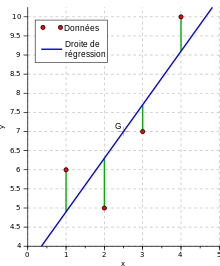
\includegraphics[scale = 0.5]{images/regression_lineaire}
% 	\caption{Graphique d'une régression linéaire classique}
% 	\label{fig:regression_lineaire}
% \end{figure}
%  
% les valeurs Y représente les résultats correspondant aux données de X et $\beta$ Les poids qui permettent de minimiser l'erreur de l'estimation, c'est à dire faire en sorte que la droite passe au plus prés possible de tous les points. 
% La formule de la régression linéaire est la suivante (à 1 dimension): 
% \begin{equation}
% Y = X * \beta + \epsilon
% \end{equation}
% $\epsilon$ est ici un nombre infiniment petit qui représente une variation minime sur tout estimateur car l'erreur est humaine et l'apprentissage aussi. 
% Cette formule nous permet facilement d'isoler $\beta$ afin de le calculer. 
% 
% En ce qui nous concerne, Y correspond à une matrice de dimension n ligne et une colonne. X représente une matrice de n ligne et p colonne ainsi $\beta$ représente une matrice à 1 ligne et p colonne. 
% Donc notre régression se calcul non pas sur une dimension mais sur n dimension. La formule devient donc :
% \begin{equation}
% Y = X_{1} * \beta_{1} +X_{2} * \beta_{2} + X_{3} * \beta_{3} + ... + \epsilon
% \end{equation}
% 
% 
% En nous basant sur cette formule, il est facile après d'isoler les $\beta_{i}$ et de les calculés. 

Une fois les paramètres estimés, il faut que le Y calculé soit entre 0 et 1. Or, les résultats donnés par la régression linéaire sont définis sur l'ensemble des réels. On applique donc une fonction logistique afin de classer les résultats. 
Ce modèle nous assure un bon ratio des résultats d'apprentissage et de test. Ainsi, nous évitons le problème de sur-apprentissage. 
Ce modèle repose sur des "pénalités". Ces pénalités sont ce que l'on peut appeler des contraintes de parcimonies qui consiste à ce que l'algorithme d'apprentissage apprenne en utilisant le moins de variables descriptives possibles. Ces contraintes permettent à l'algorithme d'éviter de rentrer en sur-apprentissage et aussi de mieux classés les voxels afin d'obtenir une meilleure classification.
\section{Validation Croisée}

La validation croisée est une méthode d'évaluation qui consiste à moyenner les scores calculés sur plusieurs jeux de données pour un seul tuple (jeu) de paramètres (voir~\autoref{fig:Valid_Croisee}).

\begin{figure}[htpb]
	\centering
	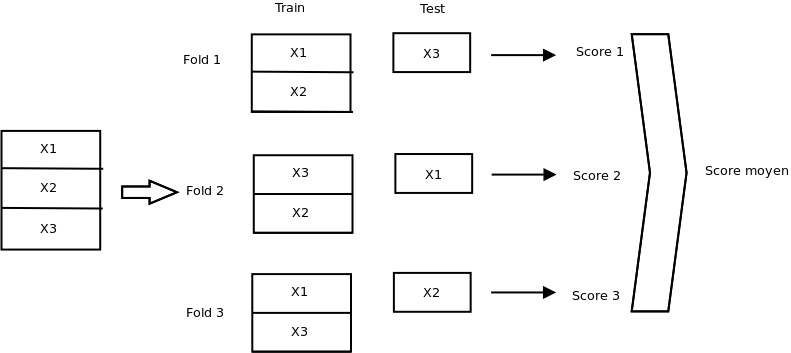
\includegraphics[scale = 0.25]{images/Valid_Croisee_param}
	\caption{Schéma de calcul d'un score par validation croisée}
	\label{fig:Valid_Croisee}
\end{figure}


Le principe de la validation croisée est de séparer un ensemble de données en plusieurs groupes de tailles équivalentes.
Sur le schéma de la  \autoref{fig:Valid_Croisee}, on peut observer un ensemble de données séparé en 3 avec $X_{1}$, $X_{2}$, $X_{3}$.
Chacun à tour de rôle sera utilisé pour l'apprentissage et le test. 
Sur les deux schémas, on peut lire "score", cela représente le résultat de la comparaison entre les prédictions et les vrais résultats par la régression linéaire. Ce score déterminera si notre prédiction est satisfaisante ou non. 

\begin{figure}[htpb]
	\centering
	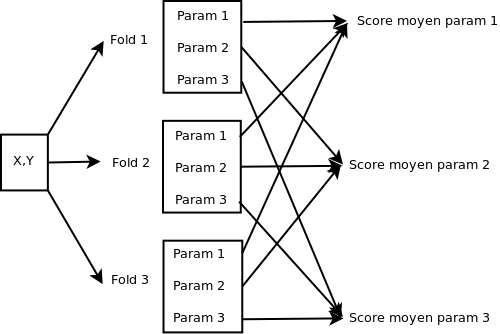
\includegraphics[scale = 0.25]{images/Valid_Croisee}
	\caption{Schéma de fonctionnement de la validation croisée}
	\label{fig:Valid_Croisee_param}
\end{figure}

Dans notre cas, les données seront diviser en 5 groupes qui tourneront à tour de rôle entre groupe d'apprentissage et groupe de test. 

Cette validation croisée est nécessaire dû à la faible quantité de sujets pour la recherche. Si nous avions 1000 sujets, cette méthode ne serait pas effectué mais pour obtenir un score assez précis pour être exploité, il nous faut cette validation croisée qui va nous donner un score de comparaison sur non pas sur 200 sujets mais sur 5 combinaisons possibles de ces 200 sujets. 

Toutes les méthodes décrites dans cette partie représentent énormément de temps de calculs.
Pour réduire ce temps, le module MapReduce va être utilisé. 
\section{MapReduce}

\subsection{Présentation générale}

MapReduce est un modèle d'architecture de développement informatique, proposé par Google, utilisé pour effectuer des calculs parallèles sur des données potentiellement très volumineuses.
Ce modèle comprend deux étapes :
\begin{itemize}
	\item map
	\item reduce
\end{itemize}

\subsubsection{Map}

Dans l'étape Map le nœud (voir~\autoref{fig:MapReduce}) analyse un problème, le découpe en sous-problèmes qu'il délègue à d'autres nœuds (qui peuvent en faire de même récursivement).
Les sous-problèmes sont ensuite traités par les différents nœuds à l'aide de la fonction Map qui à un couple (clé, valeur) associe un ensemble de nouveaux couples (clé, valeur):

\begin{equation}
map(key1,value1) → list(key2,value2)
\end{equation}

\subsubsection{Reduce}

Dans l'étape Reduce, les nœuds (voir~\autoref{fig:MapReduce}) les plus bas font remonter leurs résultats au nœud parent qui les avait sollicités.
Celui-ci calcule un résultat partiel à l'aide de la fonction Reduce (réduction) qui associe à une unique paire (clé, valeur) toutes les valeurs correspondantes à la même clé .
Puis il remonte l'information à son tour.
À la fin du processus, le nœud d'origine peut recomposer une réponse au problème qui lui avait été soumis :

\begin{equation}
reduce(key2,list(value2))→ list(value2)
\end{equation}

\begin{figure}[htpb]
	\centering
	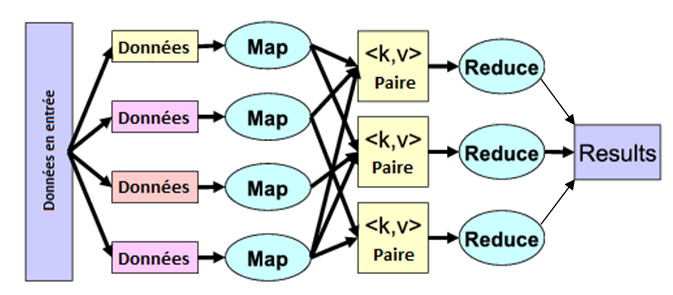
\includegraphics[scale = 0.5]{images/Mapreduce}
	\caption{Schéma de fonctionnement du MapReduce (source wikipedia)}
	\label{fig:MapReduce}
\end{figure}

\subsection{Implémentation utilisée}

Dans notre cas, nous utilisons une implémentation de MapReduce réalisée à NeuroSpin.

Dans notre cas, l'étape Map ne découpe pas nos données en plusieurs groupes, cependant elle appelle plusieurs fois la fonction de calcul des prédictions sur plusieurs clés de paramètres différents tous indépendants les uns des autres. C'est pourquoi MapReduce est utilisé afin de lancer les calculs (qui sont importants et qui prennent du temps) en parallèle sur le cluster. 

%\subsubsection{Sensibilité et spécificité: explication}

%Au dessus, on a mentionné la sensibilité et la spécificité. mots d'une grande importance qui doivent être explicité afin de bien comprendre les résultats qui vous seront présenté aprés. 
%Ces termes vient d'une technique d'analyse statistique : \textit{Receiver Operating Characteristic curve}. Cette technique  permet de classé des résultats binaires (0 ou 1) en quatre groupes sous-jacent : 
%\begin{itemize}
%	\item vrai positif
%	\item faux positif
%	\item vrai négatif
%	\item faux négatif
%\end{itemize}

%Il s'agit donc de classer des résultats entre 0 ou 1 en comparant les scores obtenus avec les vrais. Ceci forme une courbe (voir figure X) qui représente la valeur de seuil selon la spécificité et la sensibilité. 
%Ces termes ont pour historique la détection sur des radars. Les radars sont dis sensibles si ils détectent correctement les événements importants parmi les événements qu'il a détecté. En revanche, un radar est spécifique si il ne détecte que des événements importants même si il n'en détecte pas beaucoup.  
%Dans notre cas, nous nous dirons sensibles si parmi tous les sujets classés malades, tous le sont, au contraire, nous serons spécifiques si nous avons classés peu de sujet malade mais ceux qui sont classés sont vraiment malade.
%La sensibilité correspond donc au taux de vrais positifs bien classés alors que la spécificité correspond au taux de vrais négatifs bien classés.  


%Maintenant que nous savons comment sont effectués les calculs et notre classification, passons maintenant a l'analyse de nos résultats. 

\chapter{La mise en œuvre}

\section{Les sujets}

Cette étape va concerner l'initialisation de nos sujets. Comment ils ont été choisi, quels sont les spécificités, etc...

\subsection{Le choix des participants}

Les participants a ce projet ont été recruté dans trois sites différents : 
\begin{itemize}
	\item Assistance Publique-Hôpitaux de Paris Hôpital Henri Mondor-Albert Chenevier à Créteil, Fernand Widal-Lariboisière à Paris, France
	\item Western Psychiatric Institute and Clinic in Pittsburgh, Pennsylvania
	\item Central Institute for Mental Health in Mannheim, Germany, une fondation publique associée a l'université de Heidelberg.
\end{itemize}
les sujets témoins ont été recrutés parmi des contrôles, des annonces médiatiques ou encore dans des bureaux d'enregistrement parmi les trois sites. Ils ont tous été soumis à des tests reconnus pour les troubles mentaux et non aucun membre de leur famille sujet a ces mêmes troubles. Un autre critère de sélection est qu'aucun des participants n'a subi de traumatisme neurologique, n'ai une contre indication pour l'IRM.


\subsection{L'acquisition de donnée}

Toute les données ont été acquises par le même logiciel d'acquisition avec une machine IRM 3T qui ont toutes été paramétrés de la même manière sur les 3 sites. Par la suite, les images ont été normalisés et corrigés si besoin à l'aide de logiciel libre.

\todo{inclure un petit schéma concernant le prétraitement des données}

\subsection{L'initialisation de la population} 

Au commencement, nous avons 3 fichiers :
\begin{itemize}
	\item Le fichier qui contient les imageries de diffusion : \textit{all\_FA.nii.gz}
	\item Un autre contenant les identifiants de chaque sujet qui correspondent aux images : \textit{ID.tbss}
	\item Un dernier fichier qui correspond aux données cliniques de chaque sujet: \textit{BD\_clinic.xlsx} 
\end{itemize}

Avant tout, il faut s'assurer que les identifiants contenus dans le ID.tbss soient les mêmes que dans notre fichier clinique.
Une fois cela fait, nous sélectionnons les données cliniques qui nous intéressent pour l'étude en question. C'est à dire les données suivantes : 
\begin{itemize}
	\item L'identifiant du sujet
	\item l'état du patient : si il est bipolaire ou non
	\item l'age auquel l'IRM a été effectué
	\item le sex du sujet
	\item le site dans lequel l'acquisition a été fait. 
\end{itemize}

A la fin de toutes ces étapes, ces données sont enregistrés dans un nouveau fichier que nous appelons \textit{population.csv} que nous utiliserons tout du long du projet.


Une fois toutes ces données récupéré, les images seront traités. 
\section{Traitement des images et création des matrices pour l'algorithme d'apprentissage}

\subsection{Présentation des images}

À chaque sujet correspond une image de dimension (182, 218, 182) (voir~\autoref{fig:IRM}).
Les images sont regroupées en un seul fichier qui correspond donc à un volume 4D (3 dimensions d'une image plus une dimension pour les sujets).
En plus de ces images, on peut utiliser une étape supplémentaire de traitement appelée squelettisation (voir~\autoref{fig:IRM_skel}) qui permet de réduire les images à un ensemble de courbes.

\begin{figure}[htpb]
	\centering
	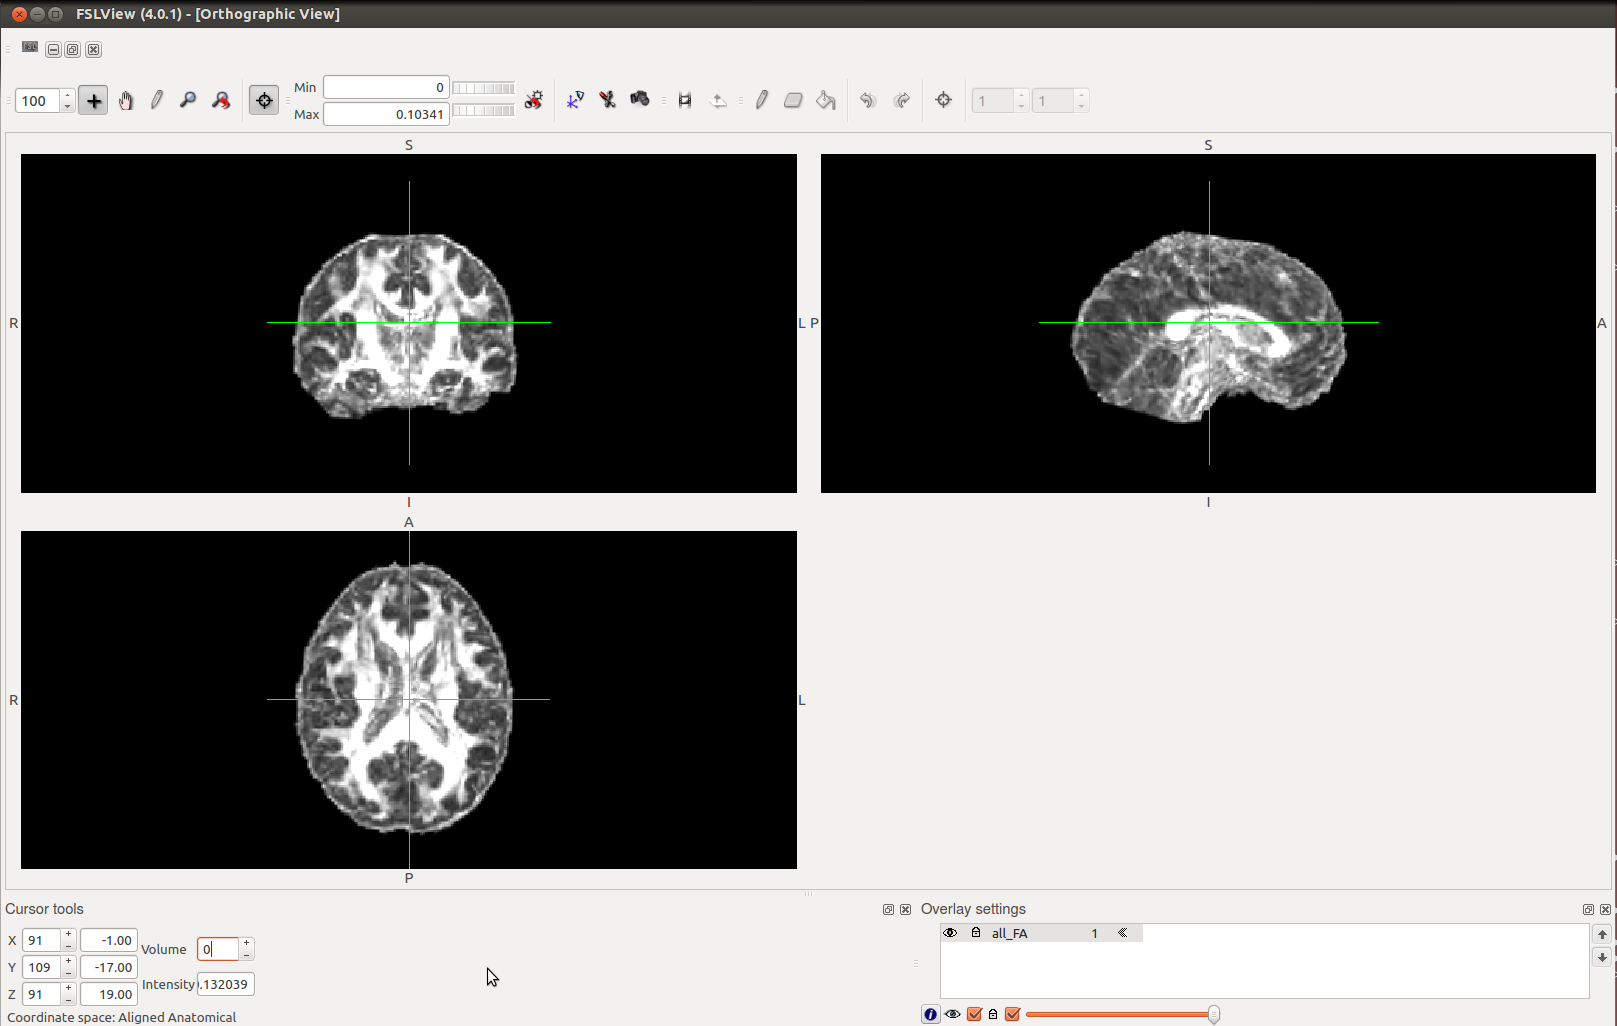
\includegraphics[scale = 0.5]{images/example_dwi}
	\caption{IRM de diffusion.}
	\label{fig:IRM}
\end{figure}

\begin{figure}[htpb]
	\centering
	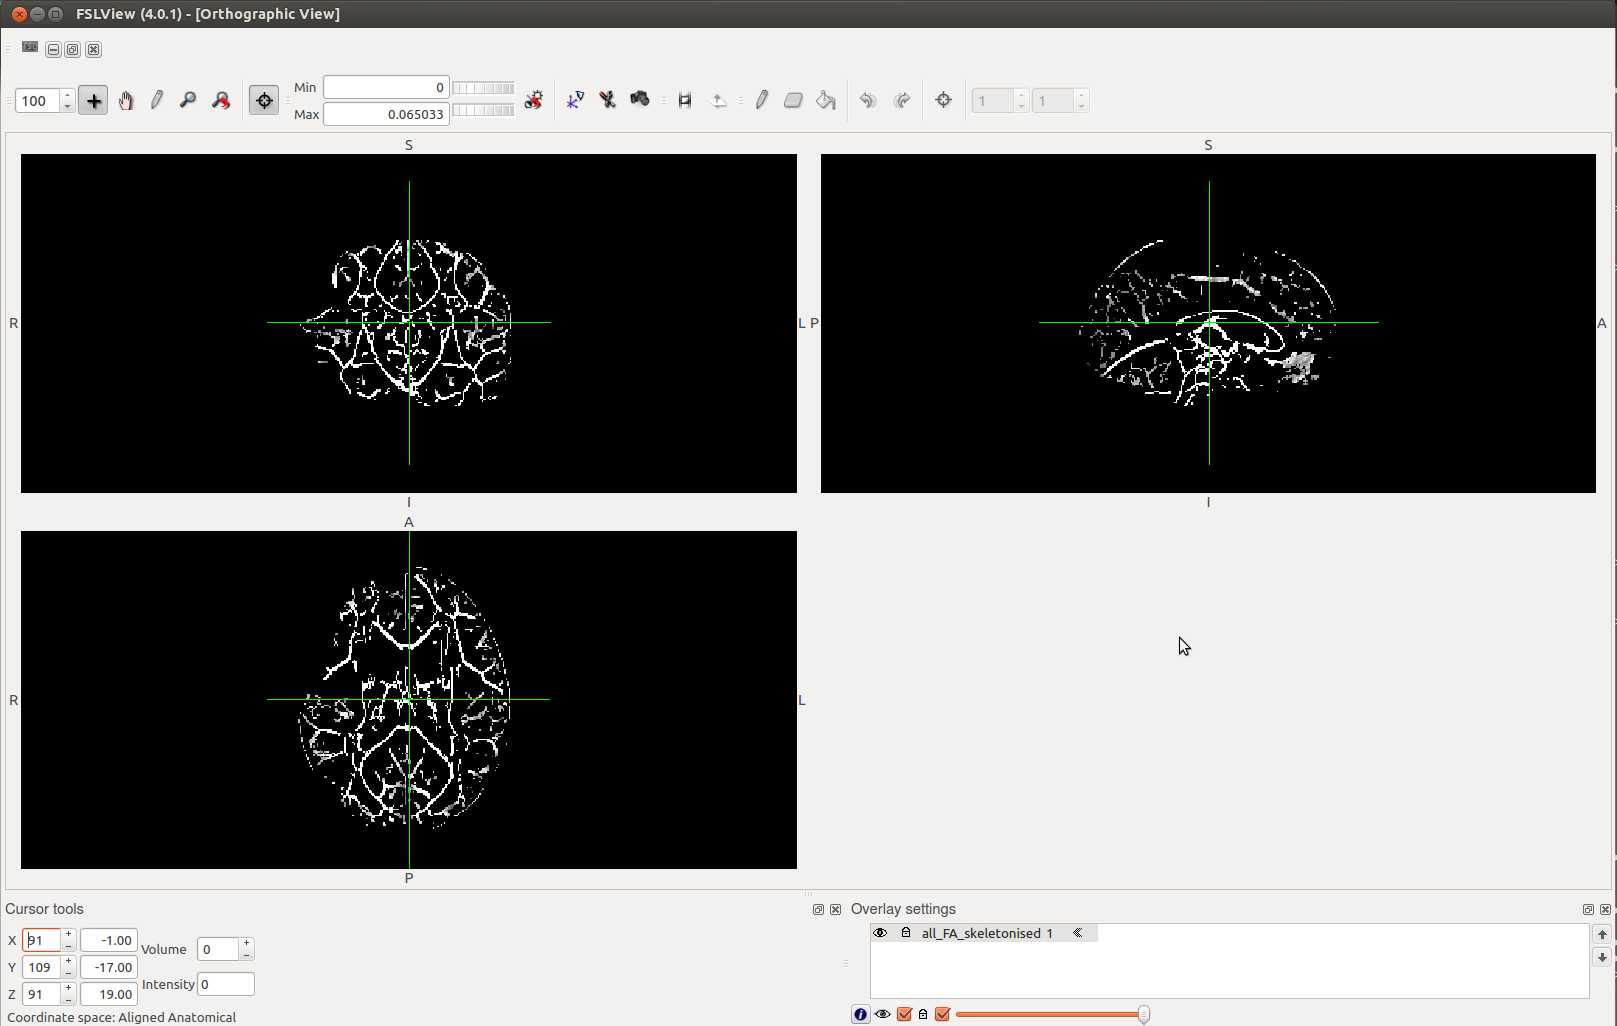
\includegraphics[scale = 0.5]{images/example_dwi_skel}
	\caption{IRM de diffusion squelettisé.}
	\label{fig:IRM_skel}
\end{figure}


\subsection{Création du masque}

Chaque image fait environ deux millions de voxels. Nous allons appliquer un masque afin de réduire le nombre de voxel et ainsi focaliser notre analyse sur une plus petite partie du cerveau. Cela nous permettra d'éliminer une grande partie des voxels qui ne nous intéressent pas. 
Ce masque (voir~\autoref{fig:masque}) sera réalisé selon les images de base avec un certain seuil suivi d'un peaufinage basé sur un atlas qui va nous permettre de sélectionner des régions du cerveau qui ne sont pas révélatrices dans notre cas. 

Dans le cas des images squelettisées (voir~\autoref{fig:masque squelétisé}), nous créons le masque sur la base de ces images. 

Dans le cas du masque tronqué (voir~\autoref{fig:mask tronqué}), nous suivons les mêmes étapes ci-dessus, suivi de l'élimination des zones du cerveau non-informatives (l'arrière du cerveau).



\begin{figure}[h]
	\centering
	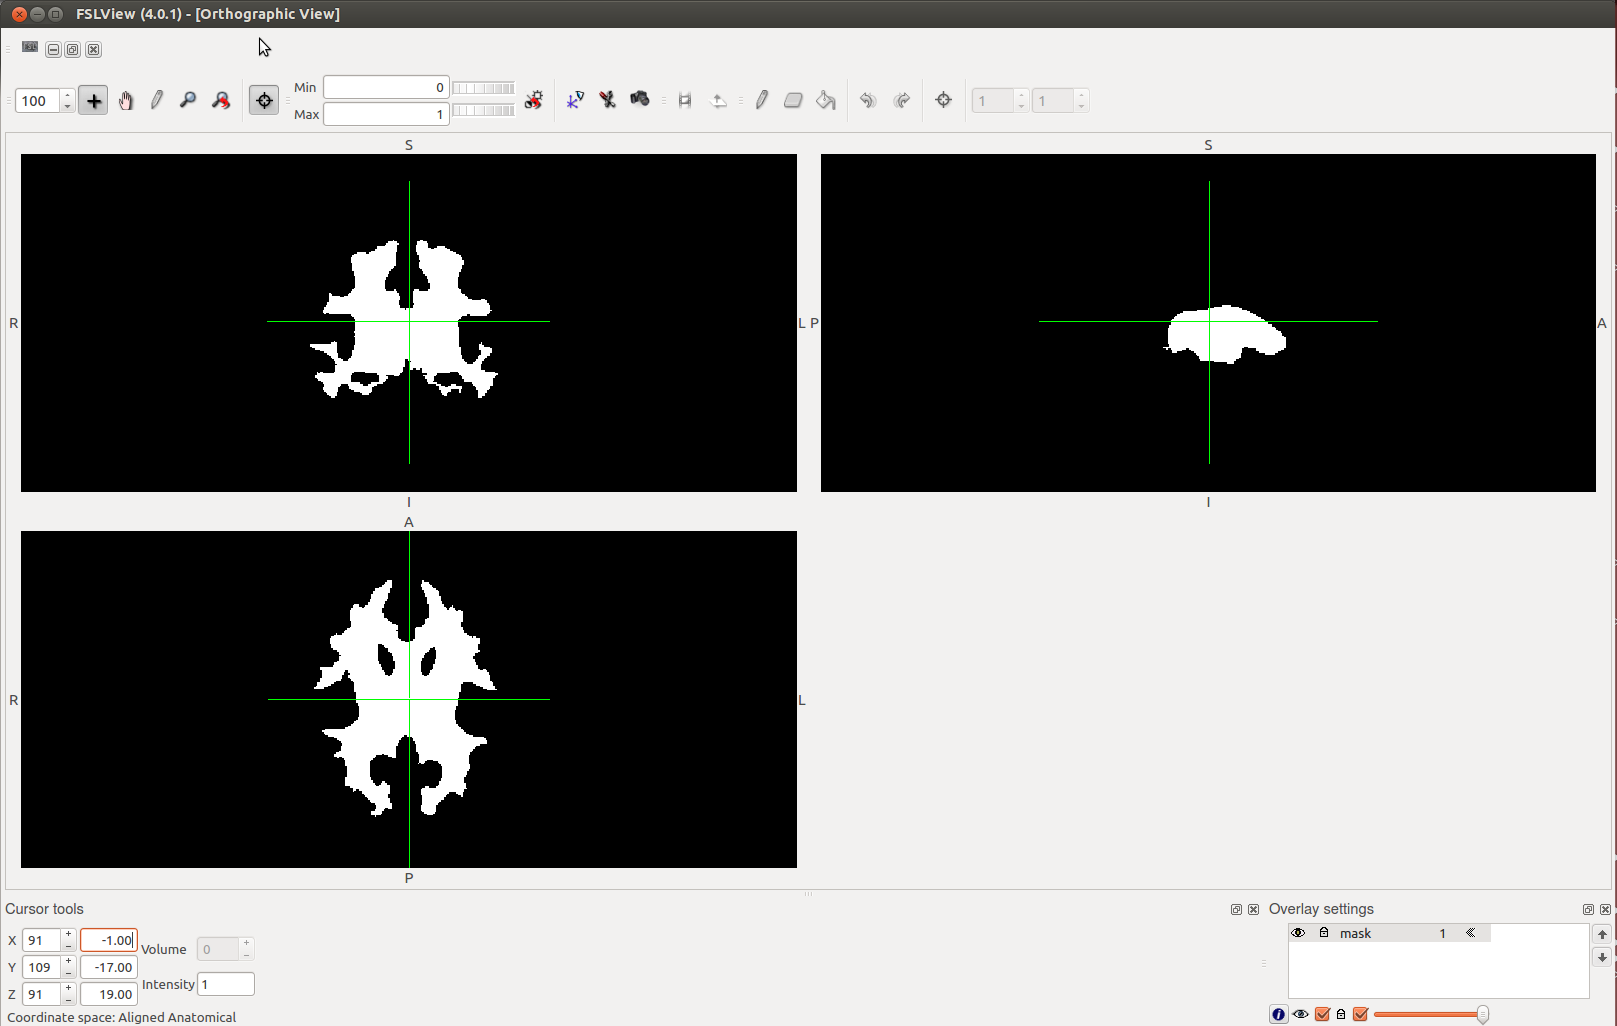
\includegraphics[scale = 0.5]{images/mask}
	\caption{Masque sans modification.}
	\label{fig:masque}
\end{figure}

\begin{figure}[h]
	\centering
	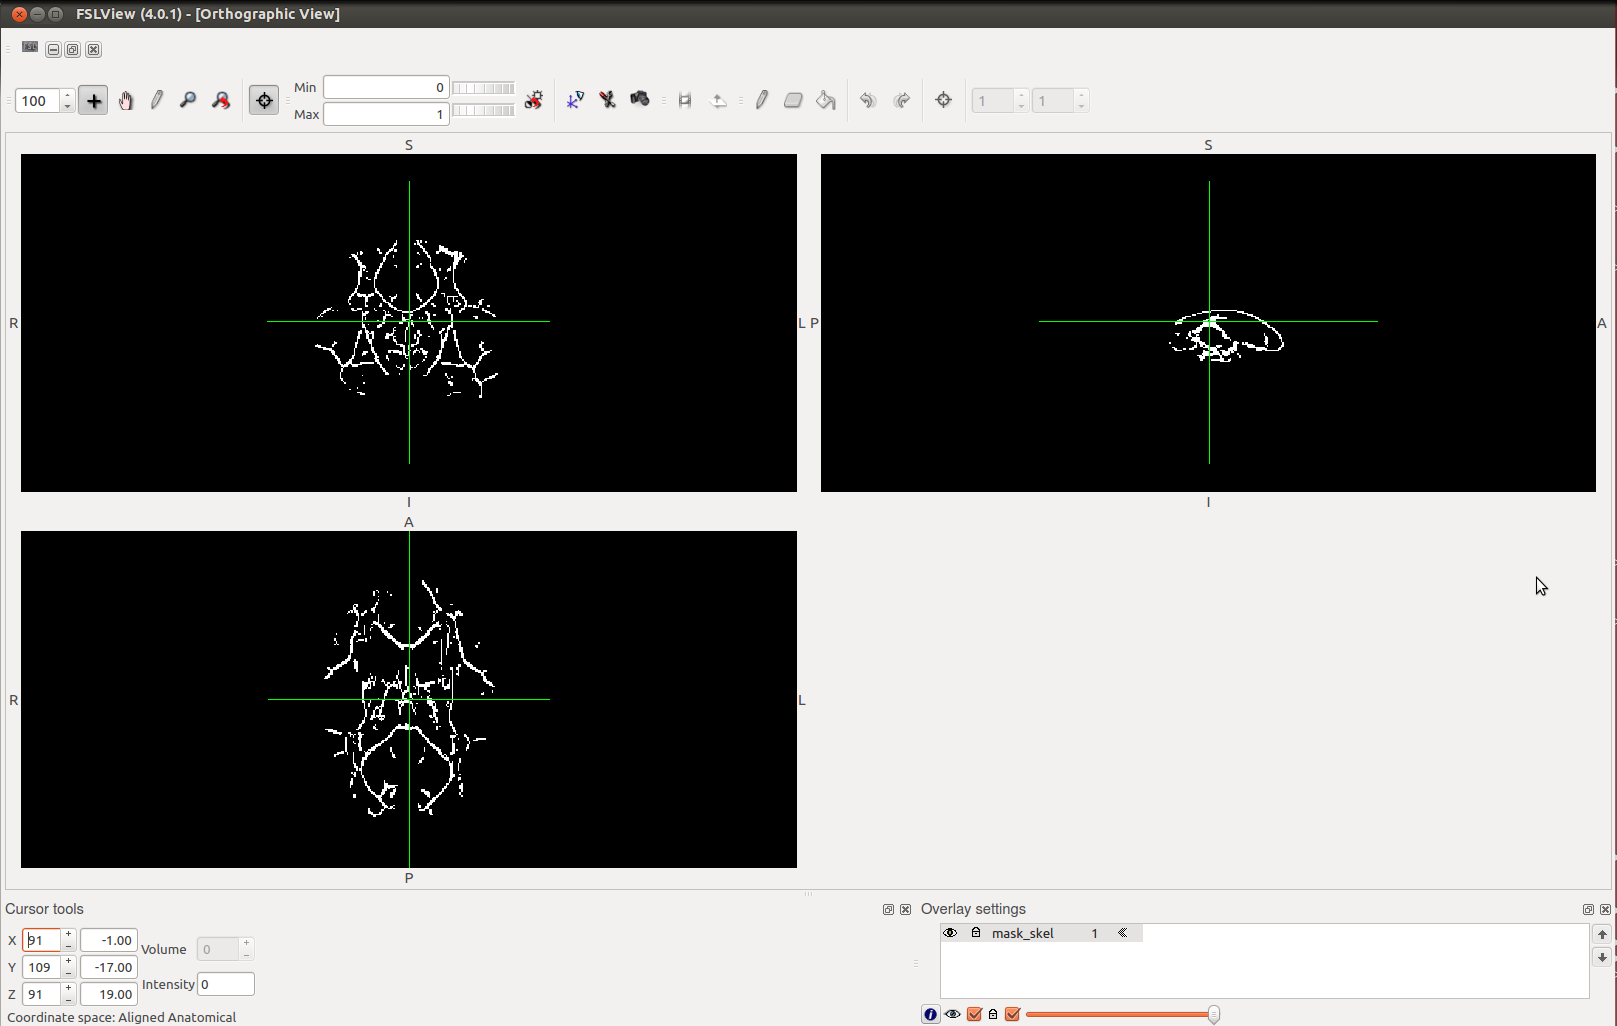
\includegraphics[scale = 0.5]{images/mask_skel}
	\caption{Masque réalisé à partir des images squelétisées.}
	\label{fig:masque squelétisé}
\end{figure}
  	
\begin{figure}[t]
	\centering
	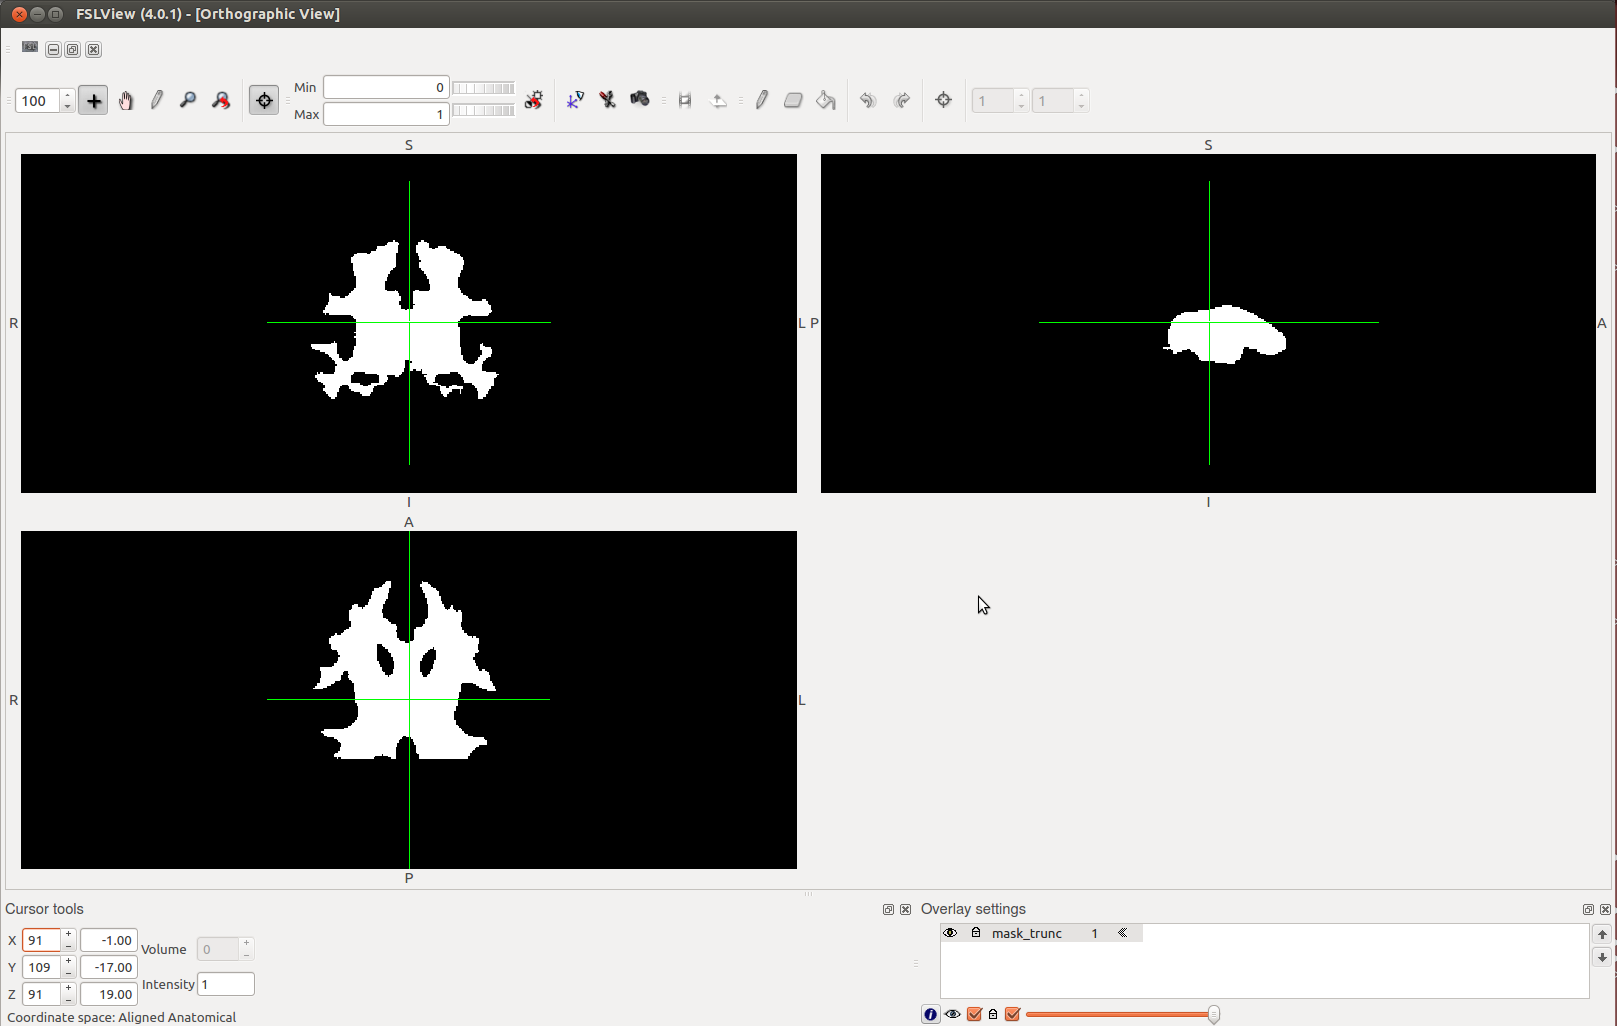
\includegraphics[scale = 0.5]{images/mask_trunk}
	\caption{Masque tronqué.}
	\label{fig:mask tronqué}
\end{figure}


\subsection{Application du masque}

Chaque image 3D est transformée en un vecteur ligne appelé \textit{vecteur d'image}.
De même, le masque est transformé en vecteur ligne.
Ce masque est utilisé pour sélectionner des éléments du vecteur.

Ainsi, nous obtenons une matrice de vecteurs où chaque ligne correspond à un sujet où le nombre de colonne correspond au nombre de voxels du masque.

Cette matrice sera ensuite centrée et réduite afin d'être normalisée. 
Cette démarche est commune à toutes les hypothèses. 

\subsection{Ajout des covariables}

Suite à la création de cette matrice, nous ajoutons des colonnes de covariables. Ces covariables sont des données cliniques qui ne seront pas pénalisées lors du calcul de prédiction. Les covariables sont le sexe des sujets et leur âge auquel a été pris l'image. 
L'âge sera centré et réduit mais pas le sexe qui sera codé en binaire (1, -1) ou le 1 correspond aux femmes et -1 les hommes. 
Ces deux colonnes sont ensuite ajoutées a la matrice X. 
Une dernière colonne est ajoutée, qui joue le rôle de l'ordonnée à l'origine et qui a pour but de diminuer l'effet biaisé (équilibrage de la classification des sujets)

Dans le cas de l'hypothèse 3, une covariable va être ajoutée, celle des sites où a été prise l'IRM. Il s'agit du \textit{Dummy Coding}, c'est à dire transformée une colonne contenant plusieurs informations qualitatives en n colonnes, une pour chaque valeur différente. 

Une autre matrice est créée, celle des Y qui correspond à l'état clinique des sujets (sain ou malade). Cette matrice est commune a toutes les hypothèses. 

Ces deux matrices seront enregistrées dans deux fichiers différents et seront utilisées lors du calcul d'apprentissage et de prédiction.


Suite à cela, nous lançons les calculs de prédiction sur un cluster. 



\section{Le calcul de prédiction}


En premier lieu, Le Mapper va distribuer les calculs avec la découpe de la population adéquate.
Ensuite l'apprentissage statistique va s'exécuter avec la régression logistique afin de calculer les scores. 
Une fois ces scores calculés, le Reducer va effectuer la validation croisée entre tous les scores pour obtenir nos prédictions finales, celles que nous analyserons plus tard. 

\subsubsection{Sensibilité et spécificité: explication}

Ci-dessus, on a mentionné la sensibilité et la spécificité. mots d'une grande importance qui doivent être explicités afin de bien comprendre les résultats qui seront présenté ensuite. 
Ces termes viennent d'une technique d'analyse statistique : \textit{Receiver Operating Characteristic curve}. Cette technique  permet de classée des résultats binaires (0 ou 1) en quatre groupes sous-jacent : 
\begin{itemize}
	\item vrai positif
	\item faux positif
	\item vrai négatif
	\item faux négatif
\end{itemize}

Il s'agit donc de classer des résultats entre 0 ou 1 en comparant les scores obtenus avec les vrais. Ceci forme une courbe qui représente la valeur de seuil selon la spécificité et la sensibilité. 
Ces termes ont pour historique la détection sur des radars. Les radars sont dits sensibles si ils détectent correctement les événements importants parmi les événements détectés. En revanche, un radar est spécifique si il ne détecte que des événements importants même si il n'en détecte pas beaucoup.  
Dans notre cas, nous nous dirons sensibles si parmi tous les sujets classés malades, tous le sont, au contraire, nous serons spécifiques si nous avons classés peu de sujet malade mais ceux qui sont classés sont vraiment malade.
La sensibilité correspond donc au taux de vrais positifs bien classés alors que la spécificité correspond au taux de vrais négatifs bien classés.  


Maintenant que nous savons comment sont effectués les calculs et notre classification, passons maintenant à l'analyse de nos résultats. 




\chapter{Analyse des résultats}

\section{Résultats de l'apprentissage selon l'hypothèse 1}

Pour rappel, l'hypothèse numéro 1 correspond aux images non modifiées avec les covariables suivantes : 
\begin{itemize}
	\item Sexe
	\item Age
	\item Site
\end{itemize}
Les résultats se présentent sous la forme d'un tableau comprenant 21 colonnes. Par souci de présentation, la totalité des résultats ne sera pas affichée mais seulement les colonnes d'importance :
\begin{itemize}
\item Paramètres
\item Sensibilité
\item Spécificité
\item Moyenne	
\end{itemize}
les 10 jeux de paramètres pour lesquels nous avons obtenus les résultats les plus probants sont rassemblés dans le tableau 1.

\begin{tabular}{|l|l|l|c|r|}
	\hline
	jeu & paramètres & Sensibilité & Spécificité & Moyenne \\
	\hline
	1 & (0.1, 0.039, 0.36, 0.601, 10000.0) & 0.616 & 0.657 & 0.636 \\
	2 & (0.5, 0.007, 0.693, 0.304, 10000.0) & 0.651 & 0.620 & 0.636 \\
	3 & (0.05, 0.039, 0.353, 0.601, 10000.0) & 0.616 & 0.648 & 0.632 \\
	4 & (0.1, 0.008, 0.792, 0.2, 10000.0) &	0.616 & 0.648 &	0.632 \\
	5 & (0.05, 0.03, 0.269, 0.701, 10000.0) & 0.651 & 0.616 & 0.631 \\
	6 & (0.01, 0.009, 0.891, 0.1, 10000.0) & 0.558 & 0.704 & 0.631 \\
	7 & (0.05, 0.399, 0.0, 0.601, 100000.0) & 0.558 & 0.704 & 0.631 \\
	8 & (0.1, 0.007, 0.693, 0.304, 10000.0) & 0.639 & 0.620 & 0.629 \\
	9 & (0.05, 0.001, 0.899, 0.1, 10000.0) & 0.546 & 0.713 & 0.629 \\
	10 & (0.1, 0.009, 0.891, 0.1, 10000.0) & 0.546 & 0.713 & 0.629 \\
	\hline
	
\end{tabular}
\\
La première colonne sont les hypers-paramètres avec lesquels nous avons effectué notre apprentissage. 
Avec l'hypothèse 1, nous obtenons une moyenne de 63\% de sujets bien classés entre non malades et malades sans différence significative entre tous les jeux de paramètres. Cette absence de différence est dûe au fait que les paramètres donnant la plus grande spécificité (n°9 et 10) sont ceux qui donnent la plus faible sensibilité et inversement (n°2 et 5). D'où la nécessité d'envisager d'autres hypothèses. 
\section{Résultats de l'apprentissage selon l'hypothèse 2 }

Pour rappel : L'hypothèse 2 est une analyse des IRM avec une troncature des parties du cerveau qui ne nous intéressent pas. Cette troncature a été faite après lecture et étude des publications déjà parues dans la littérature scientifique avec l'aide du Dr Houenou qui nous a aidé pour décider les zones du cerveau à éliminer. 
En fait, les parties éliminées sont toutes situées à l'arrière du cerveau ( cervelet, bulbe, tronc cérébral principalement). 
Les covariables sont les mêmes que pour l'hypothèse 1.
\\
Les 10 jeux de paramètres pour lesquels nous avons obtenus les meilleurs résultats sont rassemblés dans le tableau 2.

\begin{tabular}{|l|l|l|c|r|}
	\hline
	jeu & paramètres & Sensibilité & Spécificité & Moyenne \\
	\hline
	1 & (0.05, 0.196, 0.196, 0.601, -1.0) & 0.593 & 0.703 & 0.648 \\
	2 & (0.5, 0.009, 0.0898, 0.9, 100000.0) & 0.755 & 0.527 & 0.641 \\
	3 & (0.05, 0.098, 0.0, 0.9, -1.0) & 0.604 & 0.666 & 0.635 \\
	4 & (1.0, 0.009, 0.089, 0.9, -1.0) & 0.639 & 0.629 & 0.634 \\
	5 & (0.1, 0.0095, 0.941, 0.05, 100000.0) & 0.639 & 0.620 & 0.629 \\
	6 & (1.0, 0.007, 0.693, 0.304, -1.0) & 0.639 & 0.620 & 0.629 \\
	7 & (0.05, 0.45, 0.45, 0.1, -1.0) & 0.546 & 0.712 & 0.629 \\
	8 & (1.0, 0.00095, 0.949, 0.05, 100000.0) & 0.709 & 0.546 & 0.627 \\
	9 & (0.05, 0.267, 0.0299, 0.701, -1.0) & 0.569 & 0.685 & 0.627 \\
	10 & (0.05, 0.009, 0.0899, 0.9, 100000.0) & 0.744 & 0.509 & 0.626 \\
	\hline
	
\end{tabular}
\\
Ces résultats présentent plus de variabilité que ceux obtenus avec l'hypothèse précédente.
La sensibilité allant de 54\% à 75\% et la spécificité de 50\% et 71\%. Là encore, les jeux de paramètres avec la meilleure sensibilité (n°2) est le second moins spécifiques alors que les paramètres les plus spécifiques (n°7)
sont les moins sensibles.  
Cette variation n'est pas souhaitable car nous ne voulons pas avoir de doute lorsque l'on diagnostique ce genre de maladie. 
\\
La classification moyenne obtenue varie de 62\% à 64\% ce qui reste non significatif et non différent de l'hypothèse 1 d'où l'hypothèse 3.  



\section{Résultats de l'apprentissage selon l'hypothèse 3}

L'hypothèse 3 correspond à l'apprentissage sur des images squelétisées. Les covariables restent les mêmes que pour les hypothèses 1 et 2. Cette squeletisation permet un calcul plus rapide car nous prenons les voxels représentant le plus fidèlement possible les flux dans le cerveau sans pour autant prendre tous les voxels. 
\\

Les 10  jeux de paramètres pour lesquels nous obtenons les meilleurs résultats sont rassemblés dans le tableau 3.

\begin{tabular}{|l|l|l|c|r|}
	\hline
	jeu & paramètres & Sensibilité & Spécificité & Moyenne \\
	\hline
	1 & (0.01, 0.0, 0.95, 0.05, -1.0) & 0.767 & 0.564 & 0.666 \\
	2 & (0.01, 0.0, 0.99, 0.01, -1.0) & 0.802 & 0.527 & 0.665 \\
	3 & (0.01, 0.0, 0.999, 0.001, -1.0) & 0.883 & 0.425 & 0.654 \\
	4 & (0.01, 0.0, 0.99, 0.01, 100000.0) & 0.779 & 0.527 & 0.653 \\
	5 & (0.01, 0.0, 0.995, 0.005, 100000.0) & 0.813 & 0.490 & 0.652 \\
	6 & (0.01, 0.00095, 0.94905, 0.05, -1.0) & 0.732 & 0.564 & 0.648 \\
	7 & (0.01, 0.0, 0.995, 0.005, -1.0) & 0.813 & 0.481 & 0.647 \\
	8 & (0.01, 0.00095, 0.94905, 0.05, 100000.0) & 0.720 & 0.574 & 0.647 \\
	9 & (0.1, 0.0, 0.9, 0.1, -1.0) & 0.720 & 0.574 & 0.647 \\
	10 & (0.01, 0.001, 0.998, 0.001, 100000.0) & 0.848 & 0.444 & 0.646 \\
	\hline
	
\end{tabular}

Ces résultats présentent les meilleurs moyennes taux de sensibilité (72\% à 88\%), mais aussi les pires taux de spécificité (42\% à 57\%). De ce fait, les moyennes se situent au même niveau (à plus ou moins 2\% prés) que dans les deux autres cas.

\bigskip

En conclusion, à l'issu de ce travail, il est possible de proposer aux cliniciens différentes approches selon les hypothèses et les jeux de paramètres que nous venons de définir. S'ils souhaitent une grande sensibilité (détecter le plus grand nombre de malade même s'il y a quelque "faux positifs") il faudra utiliser le jeu de paramètre n°3 avec l'hypothèse 3. Par contre si c'est la spécificité qui prime, il faut utiliser le jeu n°7 de l'hypothèse 2 ou les jeux n°9 et n°10 de l'hypothèse 1.

\chapter{Ce que j'ai appris}

\end{document}